% \documentclass[compress,xcolor=table]{beamer}

% % Packages
% \usepackage[english]{babel}
% \usepackage[utf8]{inputenc}
% \usepackage[T1]{fontenc}
% \usepackage{datetime}

% % Possible options of the package (add/remove below in \usetheme call):
% %  - nosectionpages: no pages between sections
% %  - flama: use flama font, requires xelatex/lualatex + the font to compile
% %  - compressminiframes: put the heading list bullets indications pages on 1 line
% \usetheme[compressminiframes]{sorbonne}

% % Title page
% \title{Lorem Ipsum \newline Dolor Sit Amet}
% \foottitle{Lorem Ipsum Dolor Sit Amet} % optional, printed at the bottom of the slides, by default same as title, can be useful to rewrite when title has a newline for example
% \subtitle{Subtitle} % optional subtitle
% \date{\formatdate{22}{03}{2018}}
% \author{Prénom Nom}
% % \institute{LIP6 - Sorbonne Université} % Optional

% % Biblatex
% \usepackage[backend=bibtex, style=authoryear, citestyle=authoryear]{biblatex}
% \bibliography{library.bib}
% \renewcommand*{\bibfont}{\footnotesize}


% %%%%
% %% BEGIN OF SLIDES
% %%%%

% \begin{document}

% \begin{frame}[plain]
% 	\titlepage
% 	\setcounter{framenumber}{0}
% \end{frame}


\section{Data processing} \subsection{}

\begin{frame}{Data description}
	
	\begin{block}{Transaction Table}
		
		\begin{itemize}
			\item
			Taking the TransactionId as the primary key and foreign key, there are 392 characteristic variables including transaction time, transaction amount, transaction goods, etc.
		\end{itemize}
	
	\end{block}
	
	\begin{block}{Identity Table}
	    \begin{itemize}
	        \item 
	        With TransactionId as the primary key and foreign key, there are 40 characteristic variables with credit card related information.
	    \end{itemize}
			
		
	\end{block}
	
\end{frame}


\begin{frame}{Data cleaning}
	
	\begin{alertblock}{Missing values}
		
		\begin{itemize}
			\item
			According to column (attribute) statistics, if the proportion of missing value is too height, the variable will be eliminated directly;If the proportion of missing value is less than 0.2, fill with mean value or mode;In particular, for column variables with 0.2 - 0.6 missing values, the missing part is defined as a type - 1
			\item
			Count the number of attribute missing values of each sample by row. If the missing ratio is too high, it will be eliminated
		\end{itemize}
		
	\end{alertblock}
	
	\begin{block}{others}
		
		\begin{itemize}
			\item
			Remove outliers
			\item
			Eliminate constant variable
		\end{itemize}
		
	\end{block}
	
\end{frame}


\section{GAT}\subsection{}

\begin{frame}{Linear}
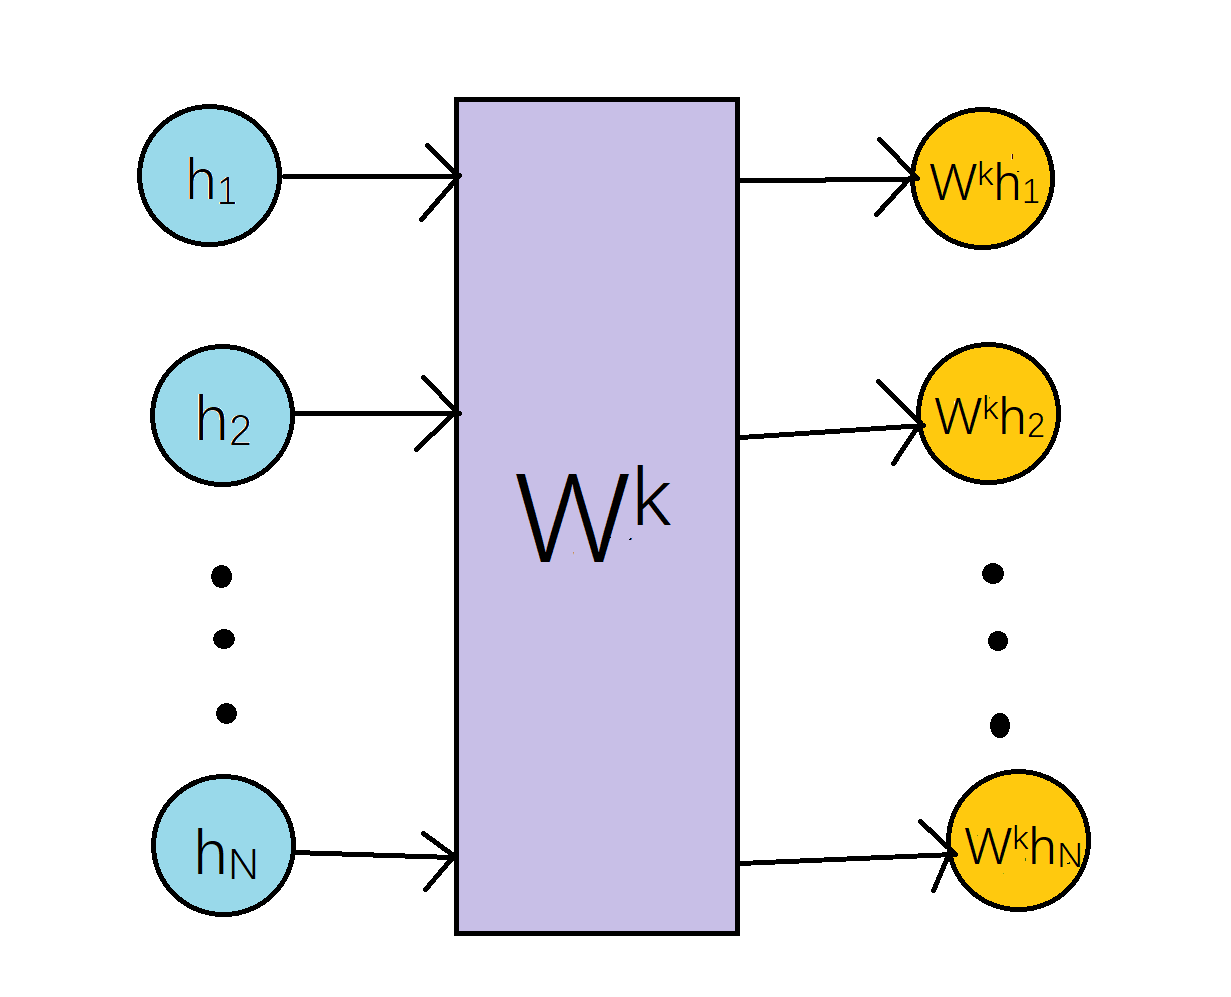
\includegraphics[width=8cm, height=4cm, scale=0.4]{images/linear.png}
\noindent\textbf{h_i\in R^{F*t}; W^k\in R^{F^{'} * F}; W^kh_i \in R^{F^{'} * t}}    
\end{frame}

\begin{frame}{attentional mechanism}
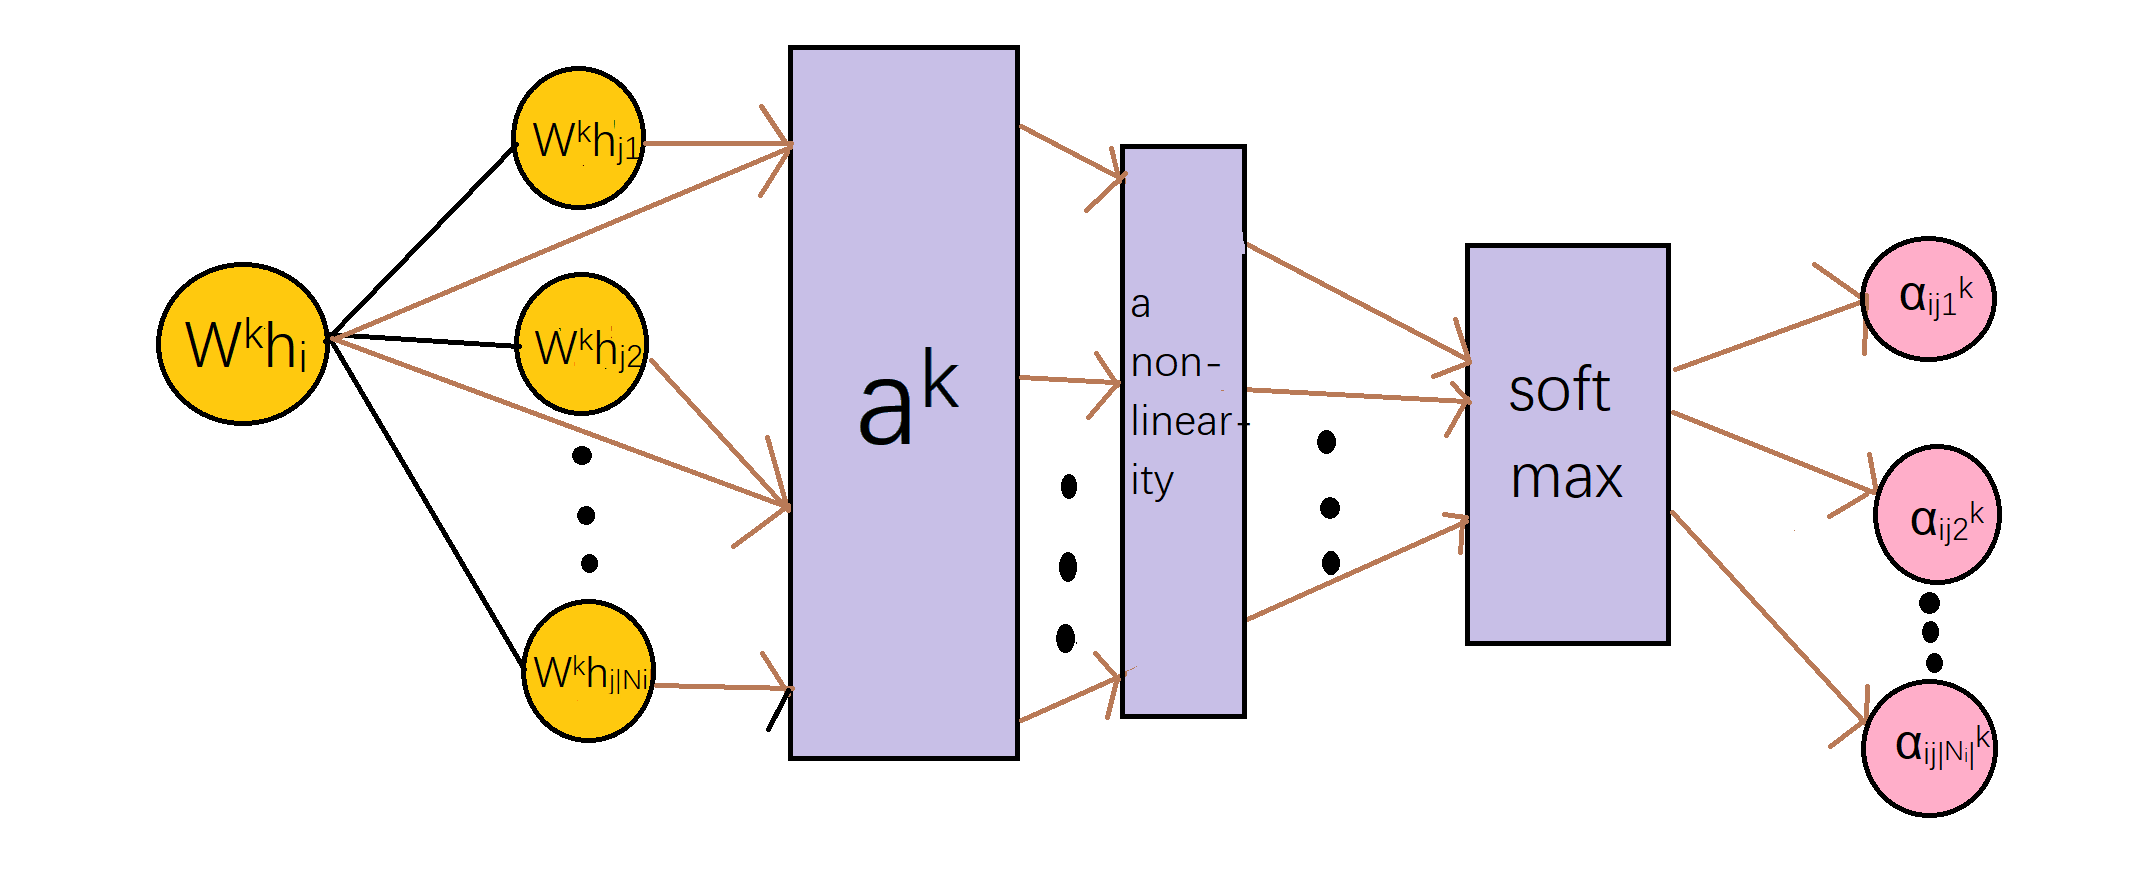
\includegraphics[width=12cm, height=6cm, scale=0.4]{images/softmax (2).png}
\noindent\textbf{W^{k}h_i \in R^{F^{'}*t}; j1, j2,...,j|N_i| \in N_i}
\noindent\textbf{N_i is neighborhood of node i(including i); a^k \in R^{2F^'}}
\end{frame}

\begin{frame}{}
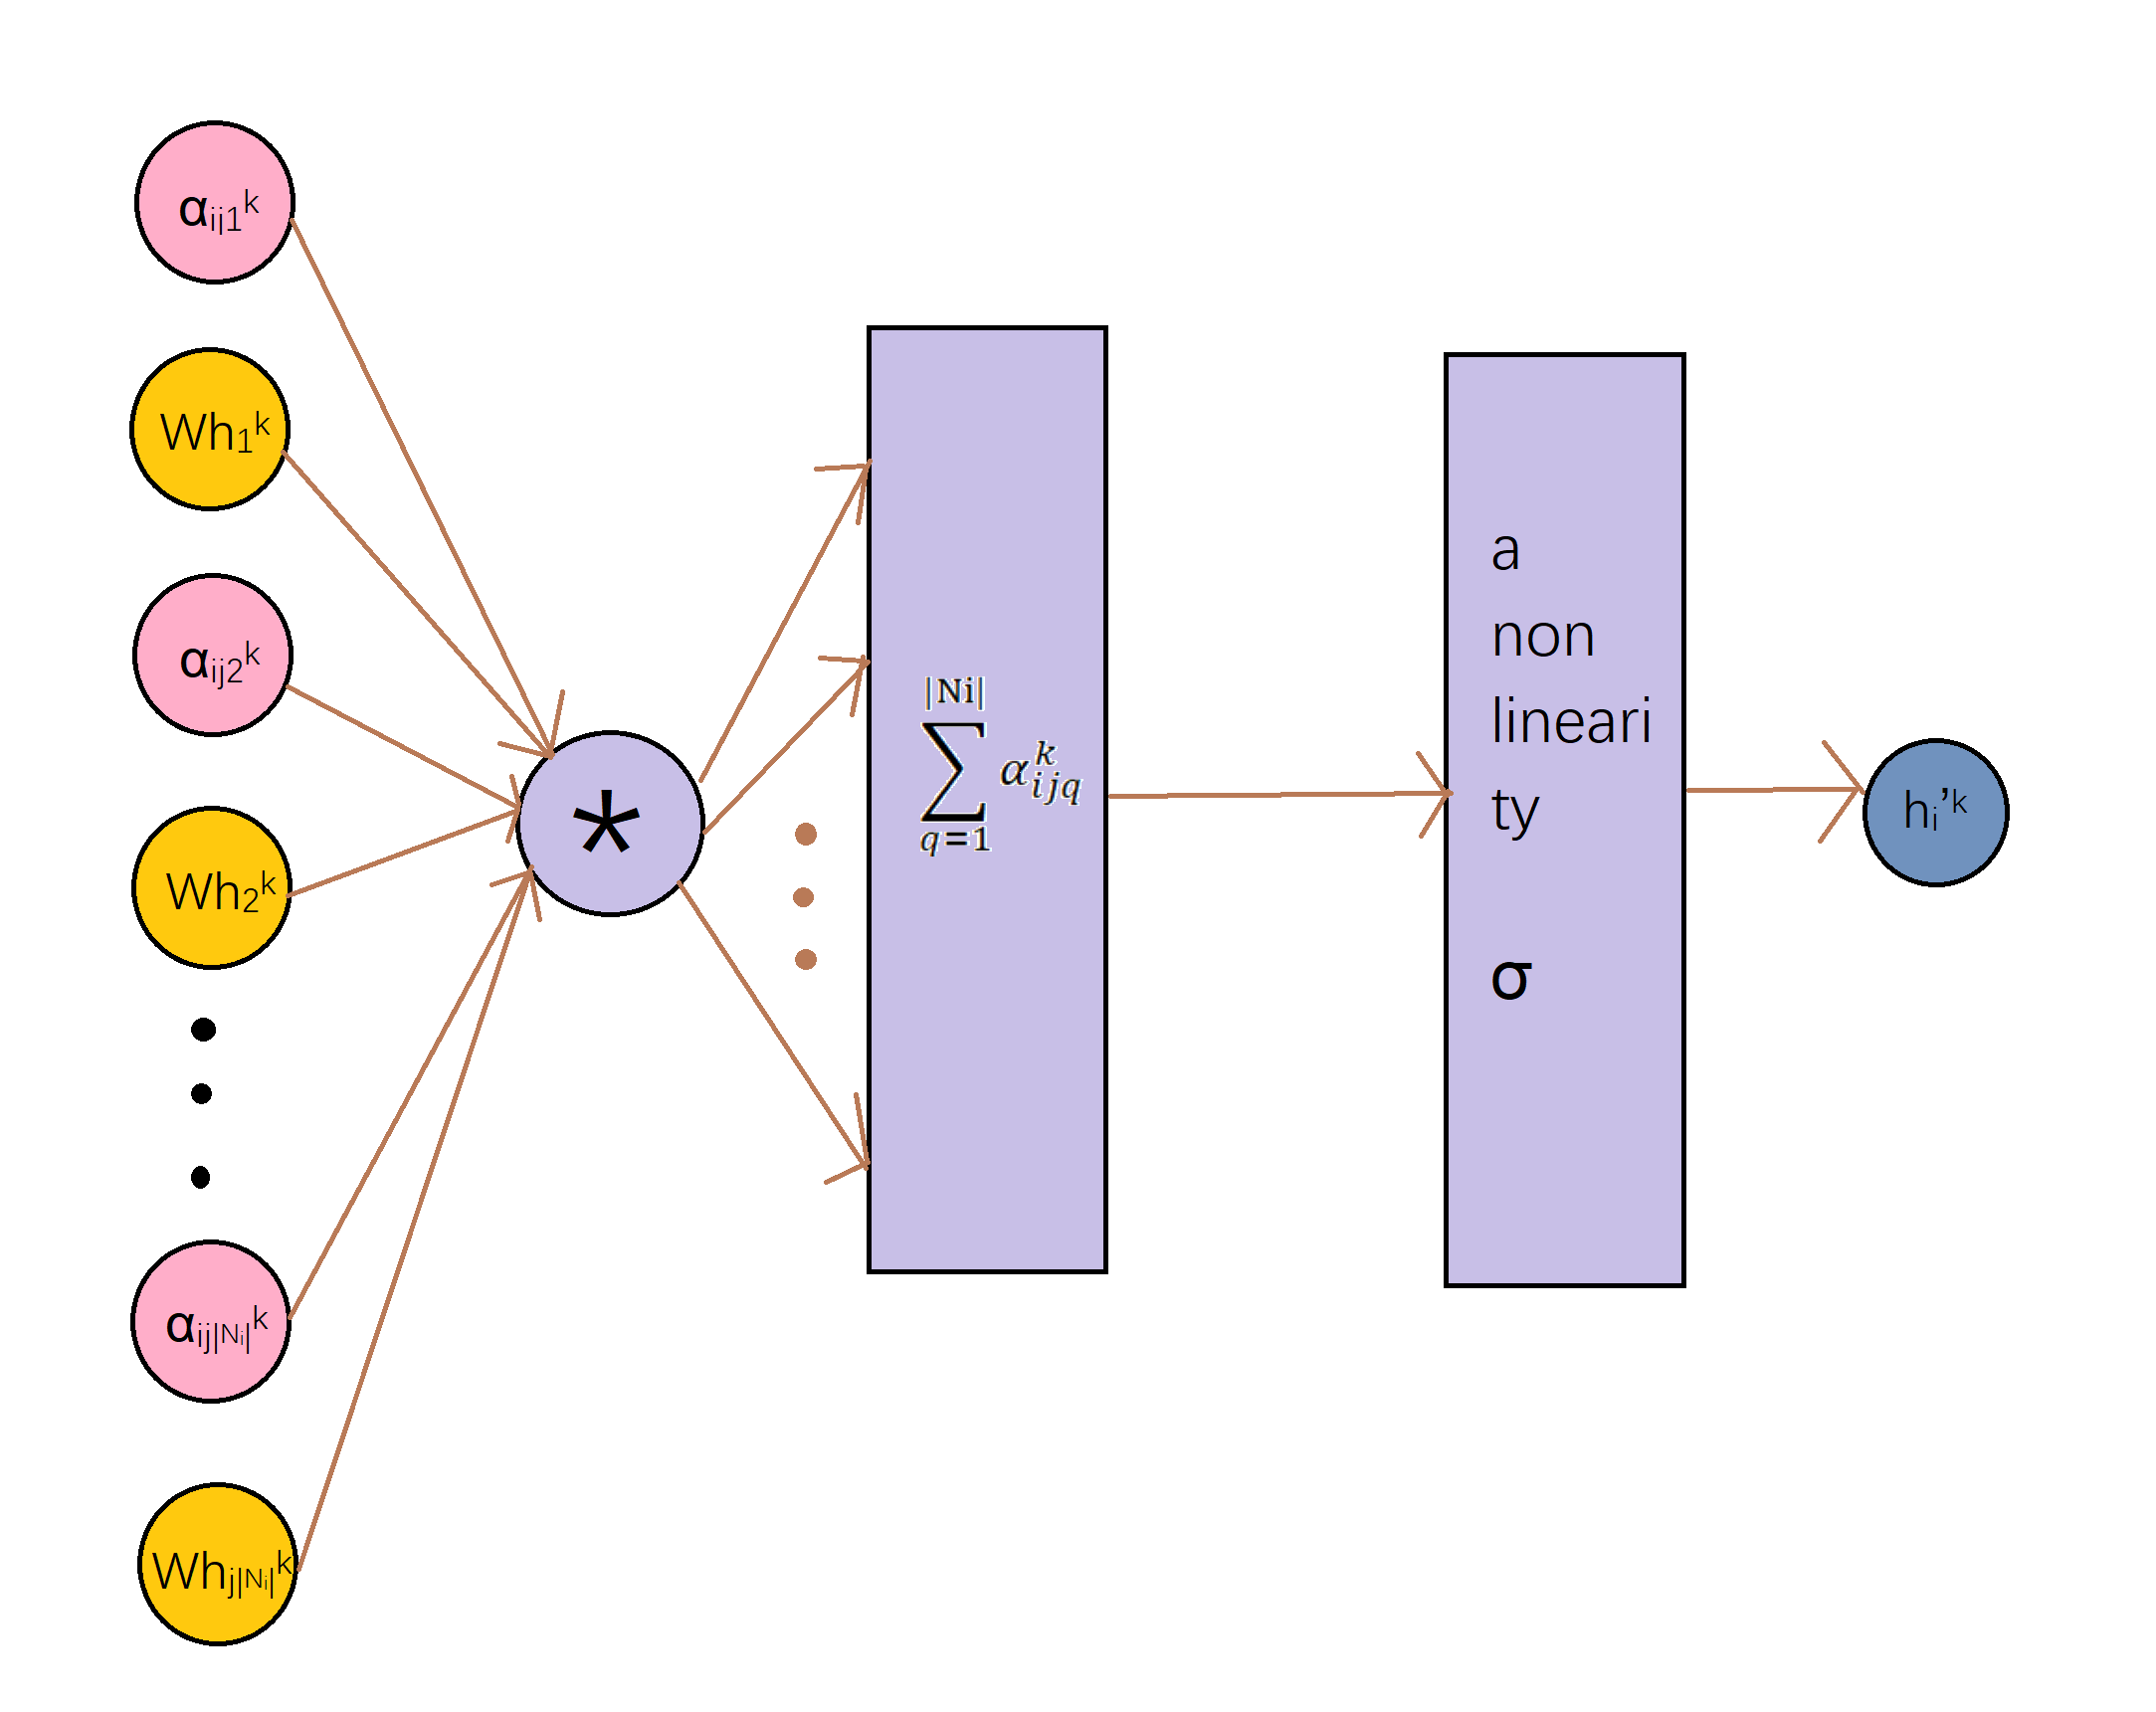
\includegraphics[width=12cm, height=6cm, scale=0.4]{images/h (2).png}
\noindent\textbf{h_i^{'k} \in R^{F^{'}*t}}
\end{frame}

\begin{frame}{}
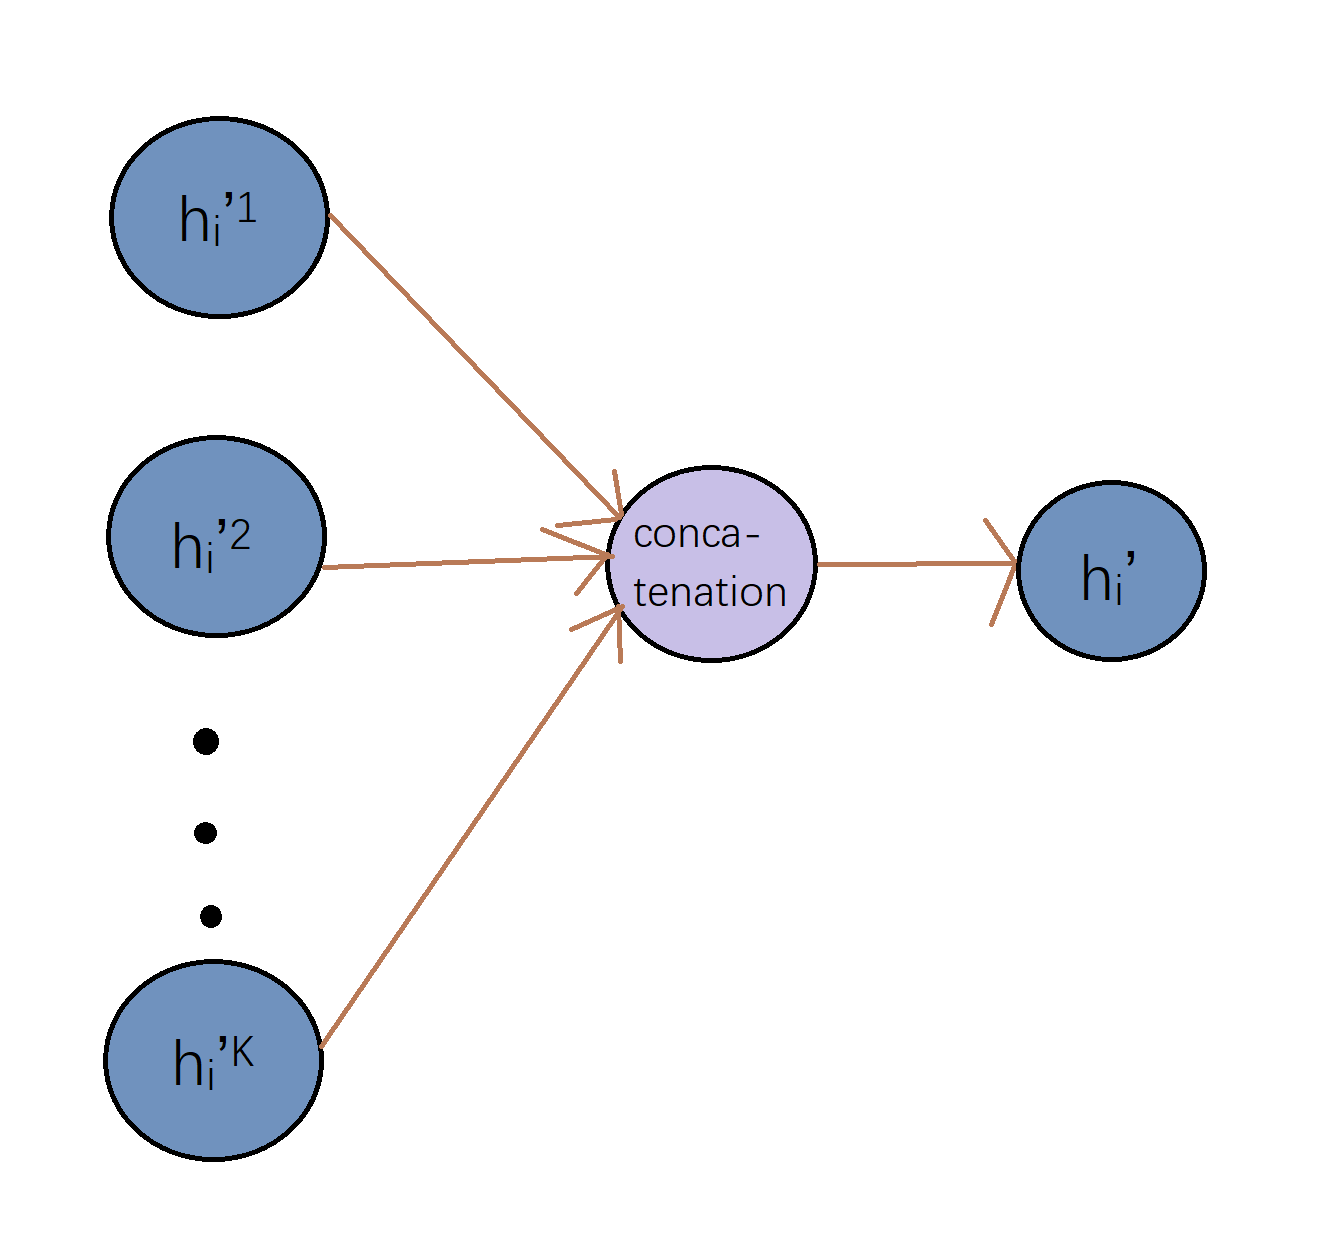
\includegraphics[width=12cm, height=6cm, scale=0.4]{images/h2 (2).png}
\noindent\textbf{h_i^' \in R^{KF^{'}*t}}
\end{frame}







% \end{document}

